\documentclass[authoryear, twocolumn]{elsarticle}
\usepackage{lmodern}
\usepackage{amssymb,amsmath}
\usepackage{ifxetex,ifluatex}
\usepackage{fixltx2e} % provides \textsubscript
\ifnum 0\ifxetex 1\fi\ifluatex 1\fi=0 % if pdftex
  \usepackage[T1]{fontenc}
  \usepackage[utf8]{inputenc}
  \usepackage{eurosym}
\else % if luatex or xelatex
  \ifxetex
    \usepackage{mathspec}
  \else
    \usepackage{fontspec}
  \fi
  \defaultfontfeatures{Ligatures=TeX,Scale=MatchLowercase}
  \newcommand{\euro}{€}
\fi
% use upquote if available, for straight quotes in verbatim environments
\IfFileExists{upquote.sty}{\usepackage{upquote}}{}
% use microtype if available
\IfFileExists{microtype.sty}{%
\usepackage{microtype}
\UseMicrotypeSet[protrusion]{basicmath} % disable protrusion for tt fonts
}{}
\usepackage[unicode=true]{hyperref}
\hypersetup{
            pdftitle={The link between tongue root advancement and the voicing effect: an ultrasound study of Italian and Polish},
            pdfauthor={Stefano Coretta},
            pdfborder={0 0 0},
            breaklinks=true}
\urlstyle{same}  % don't use monospace font for urls
\usepackage{natbib}
\bibliographystyle{plainnat}
\IfFileExists{parskip.sty}{%
\usepackage{parskip}
}{% else
\setlength{\parindent}{0pt}
\setlength{\parskip}{6pt plus 2pt minus 1pt}
}
\setlength{\emergencystretch}{3em}  % prevent overfull lines
\providecommand{\tightlist}{%
  \setlength{\itemsep}{0pt}\setlength{\parskip}{0pt}}
\setcounter{secnumdepth}{5}
% Redefines (sub)paragraphs to behave more like sections
\ifx\paragraph\undefined\else
\let\oldparagraph\paragraph
\renewcommand{\paragraph}[1]{\oldparagraph{#1}\mbox{}}
\fi
\ifx\subparagraph\undefined\else
\let\oldsubparagraph\subparagraph
\renewcommand{\subparagraph}[1]{\oldsubparagraph{#1}\mbox{}}
\fi

% set default figure placement to htbp
%\makeatletter
%\def\fps@figure{htbp}
%\makeatother

\frenchspacing
\usepackage{cleveref}
\setcitestyle{aysep={},notesep={:},citesep={,}}
\usepackage{ctable}

\title{The link between tongue root advancement and the voicing effect: an
ultrasound study of Italian and Polish}
\author{Stefano Coretta}
\date{08/09/2017}

\begin{document}
\maketitle

\section{Introduction}\label{introduction}

It is known that the root of the tongue can play a role in maintaining
voicing during the closure of voiced obstruents. The production of vocal
fold vibration requires a pressure differential between the sub-glottal
and the supra-glottal cavities (with lower pressure in the supra-glottal
cavity). During the production of voiced obstruents, the pressure in the
supra-glottal cavity quickly increases, due to the additional air
injected from the lungs in the supra-glottal cavity, which is completely
sealed in obstruent consonants. Such pressure increase can hinder the
ability to maintain voicing during closure, at the point that voicing
can stop if the lowest threshold of pressure differential is reached and
surpassed.

\citet{westbury1983} argued that one way to counterbalance the pressure
increase in the supra-glottal cavity is to enlarge the cavity through
expansion of the pharyngeal walls. One way to achieve this is to advance
the root of the tongue. \citet{ahn2016} has recently has demonstrated,
drawing from ultrasound tongue imaging, that the root of the tongue is
advanced during the articulation of voiced consonants in American
English. She also showed that tongue root advancement is present even
when vocal fold vibration is not present during closure in underlyingly
voiced stops. An interesting question arising from the connection
between voicing and tongue root is weather the advancement of the root
is correlated with other phonetic characteristics, like the duration of
vowels preceding obstruents.

An extensive pool of studies showed that vowels tend to be longer when
followed by voiced obstruents and shorter when followed by voiceless
obstruents \citep{house1953, chen1970, klatt1973, lisker1973}. Most of
the literature on the topic suggests that different languages show
different magnitudes of such durational differential, and that in some
other languages the duration of vowels is not affected by the voicing of
the following
obstruent.\footnote{For a different opinion on the first matter, see \citep{laeufer1992}.}
Although several attempts have been put forward to explain the effect of
voicing on vowel durations, no consensus has been reached to date.
Nonetheless, a recurrent theme focusses on the differences that
characterise the gestural implementation of voiced and voiceless
stops.\footnote{However, see \citep{javkin1976} and \cite{kluender1988} for two perceptually inclined proposals.}

One of the earliest articulatory accounts of the voicing effect
attributed the difference in vowel duration to the divergent
configuration of the vocal folds in sonorant and obstruent voicing
\citetext{\citealp{halle1967}; \citealp[reiterated in][]{chomsky1968}}.
According to \citet{halle1967}, voicing in obstruents is produced with a
state of the glottis that is different from the configuration necessary
to produce vocal fold vibration in sonorants like vowels. On the
contrary, they claim that voiceless stops do not require any specific
glottal configuration and thus the voicing perpetuated during the vowel
can just naturally ceases at closure (or a few milliseconds after it).
The authors thus hypothesise that, to allow the glottal state to change
from sonorant voicing to obstruent voicing, the vowel is lengthen so
that enough time is available for the change to happen.

Although such account seemed promising at the time it was proposed,
later studies failed to demonstrate that obstruent voicing is any
different from sonorant voicing {[}{]}. Given the established connection
between voicing and tongue root advancement, the hypothesis follows that
tongue root advancement could also be linked to vowel duration. If this
were the case, a language in which vowels have different durations
depending on the voicing of the following consonant should also show
tongue root advancement in voiced stops, while in those languages in
which vowel durations are not affected by voicing, tongue root
advancement should not be employed. On the same line of the hypothesis
in \citet{halle1967}, I put forward an account in which a more complex
tongue gesture in voiced consonants requires a longer time to be
achieved. A possible solution to allow for this additional time is to
maintain the vocalic gesture for a prolonged time (as in the
\citet{halle1967} hypothesis). If tongue root advancement plays a role
in determining the duration of preceding vowels through such extension
mechanism, than it is expected that languages with the voicing effect
show a systematic advancement of the tongue root in voiced stops.

In a study assessing general properties on segmental durations of spoken
Italian, \citet{farnetani1986} found that the first vowel in /lada/ was
on average 35 msec longer than the vowel in /lata/ (/lata/ 223 msec, sd
= 18; /lada/ 258 msec, sd = 13, p.~26). \citet{esposito2002} extended
Farnetanis's research to all vowels and stops and found that vowels were
longer when followed by a voiced stop, with an estimate similar to what
reported in \citet{farnetani1986}. Vowels in Polish, on the other hand,
are not affected by the voicing of the following consonant, according to
\citet{keating1984}. Italian and Polish have been chosen as the two test
languages for this study.

\section{Methodology}\label{methodology}

\subsection{Participants}\label{participants}

\ctable[caption = Sociolinguistic information on participants. The right-most column indicates whether the participant spent more than 6 consecutive months abroad.,
label = t:participants
]{lllll}{}{
\FL
\textbf{id}   & \textbf{sex} & \textbf{age} & \textbf{city}     & \textbf{\textgreater} 6 mo \ML
IT01 & m   & 28  & Verbania & yes               \NN
IT02 & m   & 26  & Udine    & yes               \NN
IT03 & f   & 27  & Verbania & no                \NN
IT04 & f   & 54  & Verbania & no                \NN
PL02 & f   & 32  & Poznań   & yes               \NN
PL03 & m   & 26  & Poznań   & yes               \NN
PL04 & f   & 34  & Warsaw   & no                \NN
PL05 & m   & 34  & Przasnysz & no               \LL
}

Eight native speakers of Italian (2 females, 2 males) and Polish (2
females, 2 males) have been recorded in Manchester and in Italy
\Cref{t:participants}. The Italian speakers were from Northern Italy
(three from the Northwest and one from Northeast). The Polish group was
more heterogeneous, with two speakers from Poznań, one from Przasnysz,
and one from Warsaw. This research has obtained ethic clearance from the
University of Manchester (REF 2016-0099-76). The participants received a
monetary compensation of £10/10\euro{}.

\subsection{Equipment set-up}\label{equipment-set-up}

\begin{figure*}
    \centering
    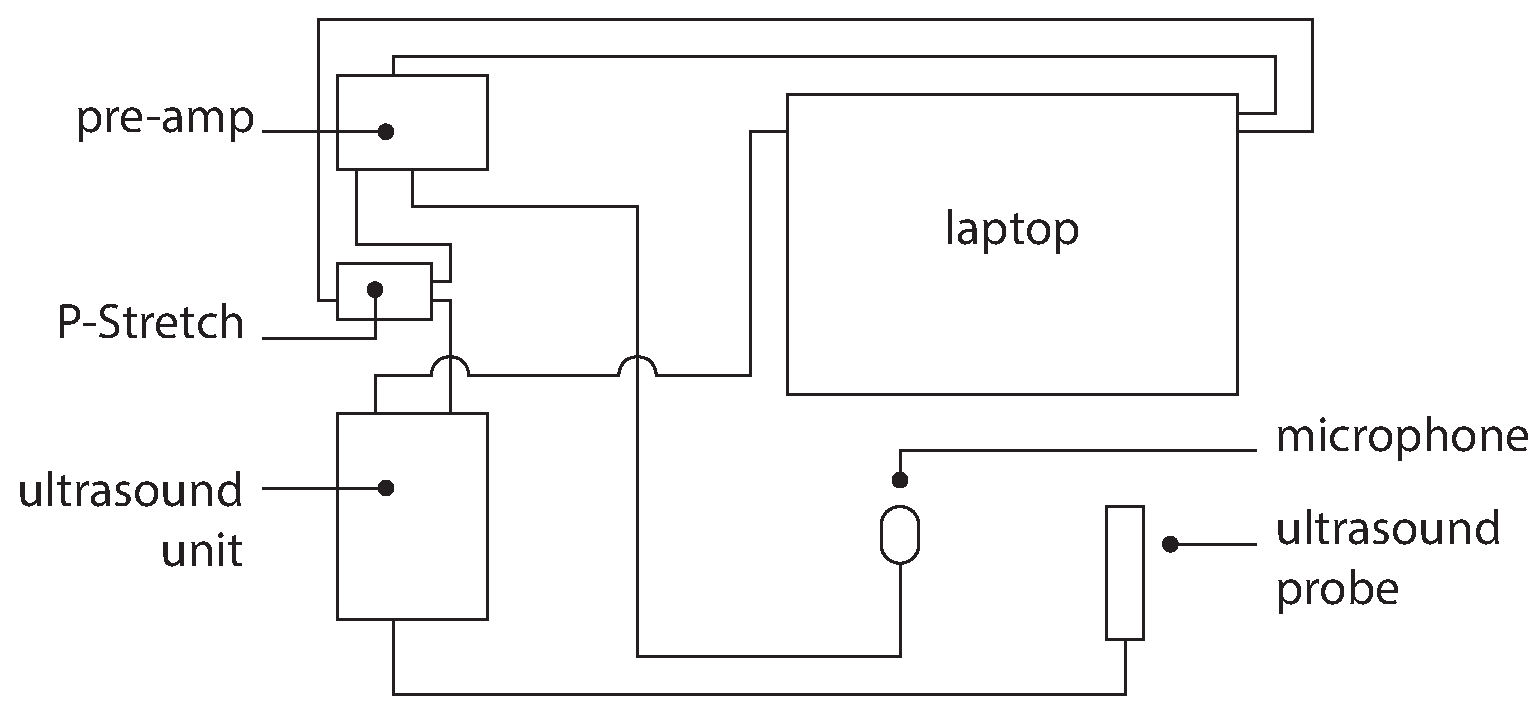
\includegraphics[width=.7\textwidth]{../../graphics/uti-setup.pdf}
    \caption{Schematic representation of the equipment setup (\citealt{articulate2011}, see text for details).}
    \label{f:uti-setup}
\end{figure*}

An Articulate Instruments Inc. set-up was used for this study
(\Cref{f:uti-setup}). This is constituted by a TELEMED Echo Blaster 128
unit with a TELEMED C3.5/20/128Z-3 ultrasonic transducer (20mm radius,
2-4 MHz). A synchronisation unit (P-Stretch) was plugged into the Echo
Blaster unit and used for automatic audio/ultrasound synchronisation. A
FocusRight pre-amplifier and a Movo LV4-O2 Lavalier microphone were used
for audio recording. The acquisition of the ultrasonic and audio signals
was achieved with the software Articulate Assistant Advanced (AAA,
v2.17.2) running on a Hawlett-Packard ProBook 6750b laptop with
Microsoft Windows 7. Finally, stabilisation of the ultrasound probe was
ensured by using a stabilisation headset produced by Articulate
Instruments Inc. (not shown in the figure).

\subsection{Materials}\label{materials}

Disyllabic words of the form
C\textsubscript{1}V\textsubscript{1}C\textsubscript{2}V\textsubscript{2}
were used as targets, where C\textsubscript{1} = /p/, V\textsubscript{1}
= /a, o, u/, C\textsubscript{2} = /t, d, k, g/, and V\textsubscript{2} =
V\textsubscript{1} (e.g. /pata/, /pada/, /poto/, etc.), yielding a total
of 12 target words. A labial stop was chosen as the first consonant to
reduce influence on the following vowel (although cf.
\citet{vazquez-alvarez2007}). Only coronal and velar stops were used as
target consonants since labial consonants cannot be imaged with
ultrasonography. The target words were embedded in a frame sentence.
Prosodically similar sentences were used to ensure comparability between
languages. The frame sentence was \emph{Dico X lentamente} `I say X
slowly' for Italian, and \emph{Mówię X teraz} `I say X now' for Polish.

\subsection{Procedure}\label{procedure}

The sentences with the target words were randomised for each
participant, although the order was kept the same between repetitions
within participant due to software constraints. Each participant
repeated the list of randomised stimuli six times. The participant
occlusal plane was obtained using a bite plate, and the hard palate was
imaged by asking the participant to swallow water \citep{scobbie2011}.
The frame rate of the acquisition of the ultrasonic data varied between
55 and 65 frames per second (one frame every 18-15 milliseconds). The
audio signal was recorded at 22050 MHz (16-bit).

\subsection{Data processing}\label{data-processing}

Synchronisation of the ultrasonic and audio signal was achieved in
post-processing, using a built-in procedure of AAA. The data were then
subjected to force alignment using the SPASS force aligner
\citep{bigi2015}. The outcome of the automatic annotation was then
manually corrected, according to the criteria in \Cref{t:dur-measures}.
The onset of the target consonant burst (C2 burst) was detected
automatically employing a Praat \citep{boersma2016} implementation of
the algorithm described in \citet{ananthapadmanabha2014}. The duration
of the following intervals was then extracted from the acoustic
landmarks using an automated procedure in Praat: vowel duration (V1
onset to V1 offset), consonant duration (V1 offset to V2 onset), and
closure duration (V1 offset to C2 burst).

\ctable[caption = List of measurements as extracted from acoustics.,
label = t:dur-measures,
width=\textwidth,
star
]{ll>{\raggedright}p{9cm}}{}{
\FL
\textbf{landmark}               &                  & \textbf{criteria}                                                                                    \ML
vowel onset           & (V1 onset)         & appearance of higher formants in the spectrogram following the burst of /p/ (C1)            \NN
vowel offset          & (V1 offset)        & disappearance of the higher formants in the spectrogram preceding the target consonant (C2) \NN
consonant onset       & (C2 onset)         & corresponds to V1 offset                                                                    \NN
closure onset         & (C2 closure onset) & corresponds to V1 offset                                                                    \NN
consonant offset      & (C2 offset)        & appearance of higher formants of the vowel following C2 (V2); corresponds to V2 onset                                \NN
consonant burst onset & (C2 burst)         & automatic detection \citep{ananthapadmanabha2014}                                           \LL
}

Tongue contours were extracted from the ultrasonic data using AAA.
Spline curves were first fitted to the visible contours using the AAA
batch tracking function. Manual correction was applied in those cases
that showed clear tracking errors. The time of maximum tongue
displacement within consonant closure was then calculated in AAA
following the method in \citet{strycharczuk2015}. Fan line selection in
this study was achieved by finding the fan line within the relevant area
of the tongue (tongue tip for coronal consonants and tongue dorsum for
velar consonants) with the highest standard deviation of displacement.

\subsection{Analysis}\label{analysis}

The tongue contours coordinates were exported at two time points: (1) at
the C2 closure onset, and (2) at maximum tongue displacement. The
contours were normalised by applying offsetting and rotation relative to
the participant's occlusal plane \citep{scobbie2011}. Generalised
additive mixed effects regression models \citep{wood2006} were used for
the statistical analysis of tongue contour data in R
\citep{r-core-team2017}. Duration measurements were subject to linear
mixed effects models using \texttt{lme4} in R \citep{bates2015}.

\section{Results}\label{results}

\subsection{Vowel duration and
voicing}\label{vowel-duration-and-voicing}

A linear mixed effect regression model was fitted on the Italian vowel
durations with duration as the outcome variable; \textsc{vowel quality}
(/a, o, u/), \textsc{voicing} and \textsc{place of articulation} of the
following consonant, \textsc{sentence duration} as fixed effects; random
intercepts by speaker and word, and by-speaker random slopes for voicing
. An interaction between voicing and vowel quality was also included in
the final model, since it turned out to be significant. P-values were
obtained through likelihood ration tests comparing the full model
including voicing with a null model without voicing as a predictor.
According to the full model, Italian vowels are 19.5 milliseconds (±5.5
standard errors) longer if followed by a voiced stop (\(\chi^2\)(3) =
18.5, p = 0.000337).

For Polish, the same model structure was used, excluding the
voicing-vowel interaction (which was not significant). Surprisingly, the
model reported a partially significant 8 milliseconds (±3 standard
errors) effect of consonantal voicing on the preceding vowel
(\(\chi^2\)(1) = 5.4, p = 0.02). The exploration of the random slopes
for each speaker indicated that PL05 showed a particularly higher slope
for voicing, meaning that the effect of voicing was stronger in his
data, with an estimated 14 milliseconds effect of voicing. This
observation will come at hand when discussing about the results of the
tongue contour data.

\subsection{Tongue contours}\label{tongue-contours}

\begin{figure*}
    \centering
    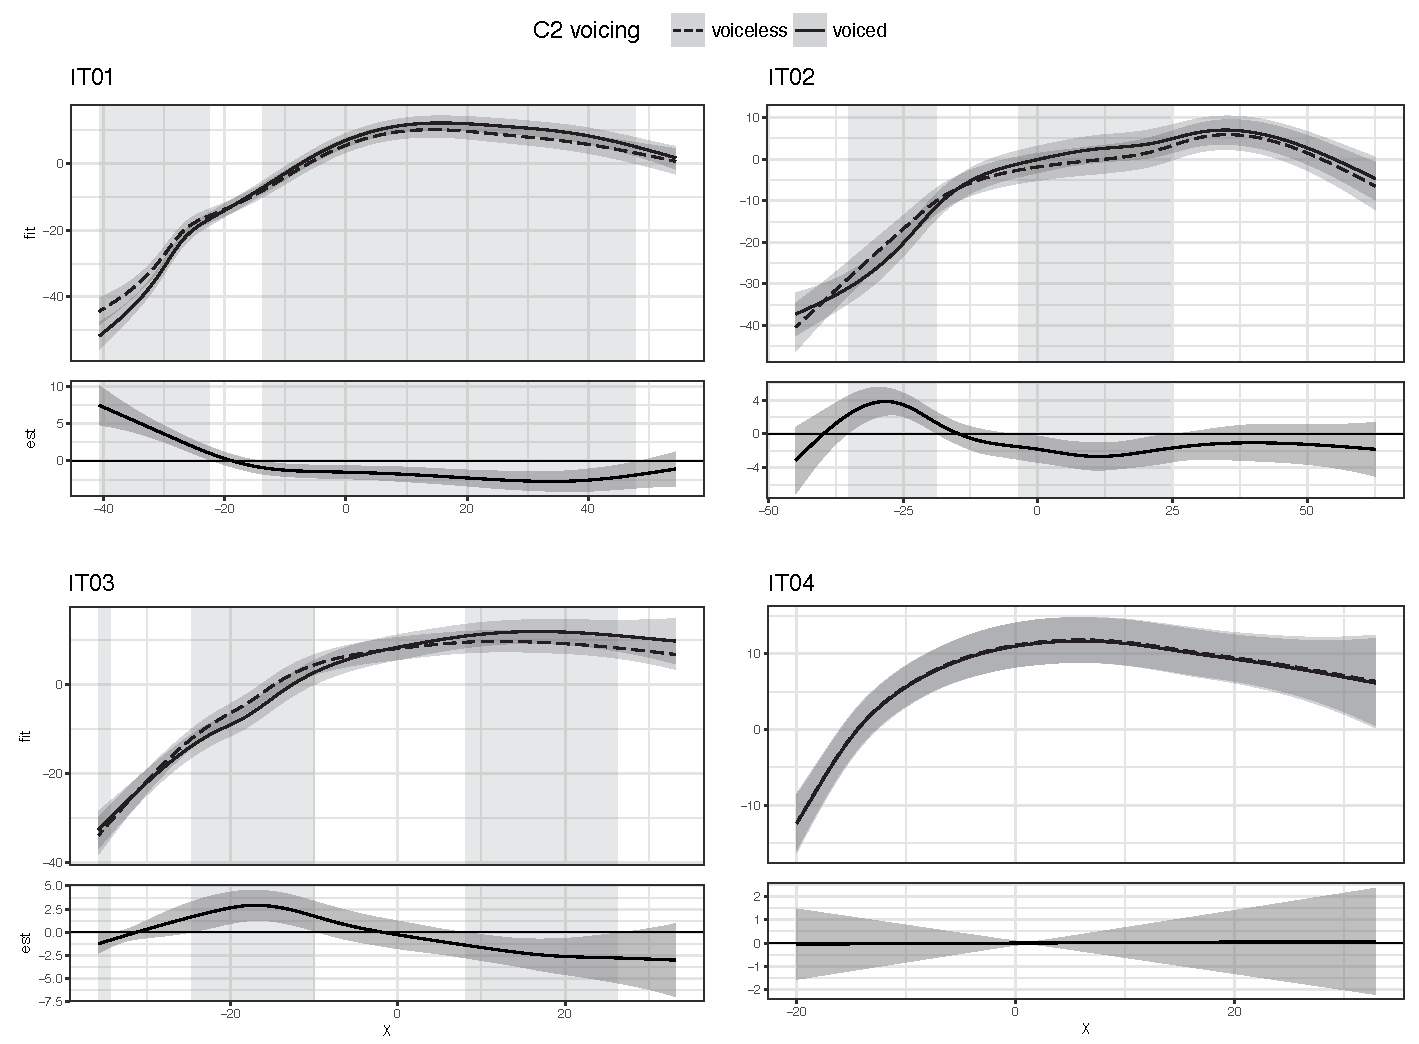
\includegraphics[width=.7\textwidth]{fig/italian-tra.pdf}
    \caption{Schematic representation of the equipment setup (\citealt{articulate2011}, see text for details).}
    \label{f:uti-setup}
\end{figure*}

\begin{figure*}
    \centering
    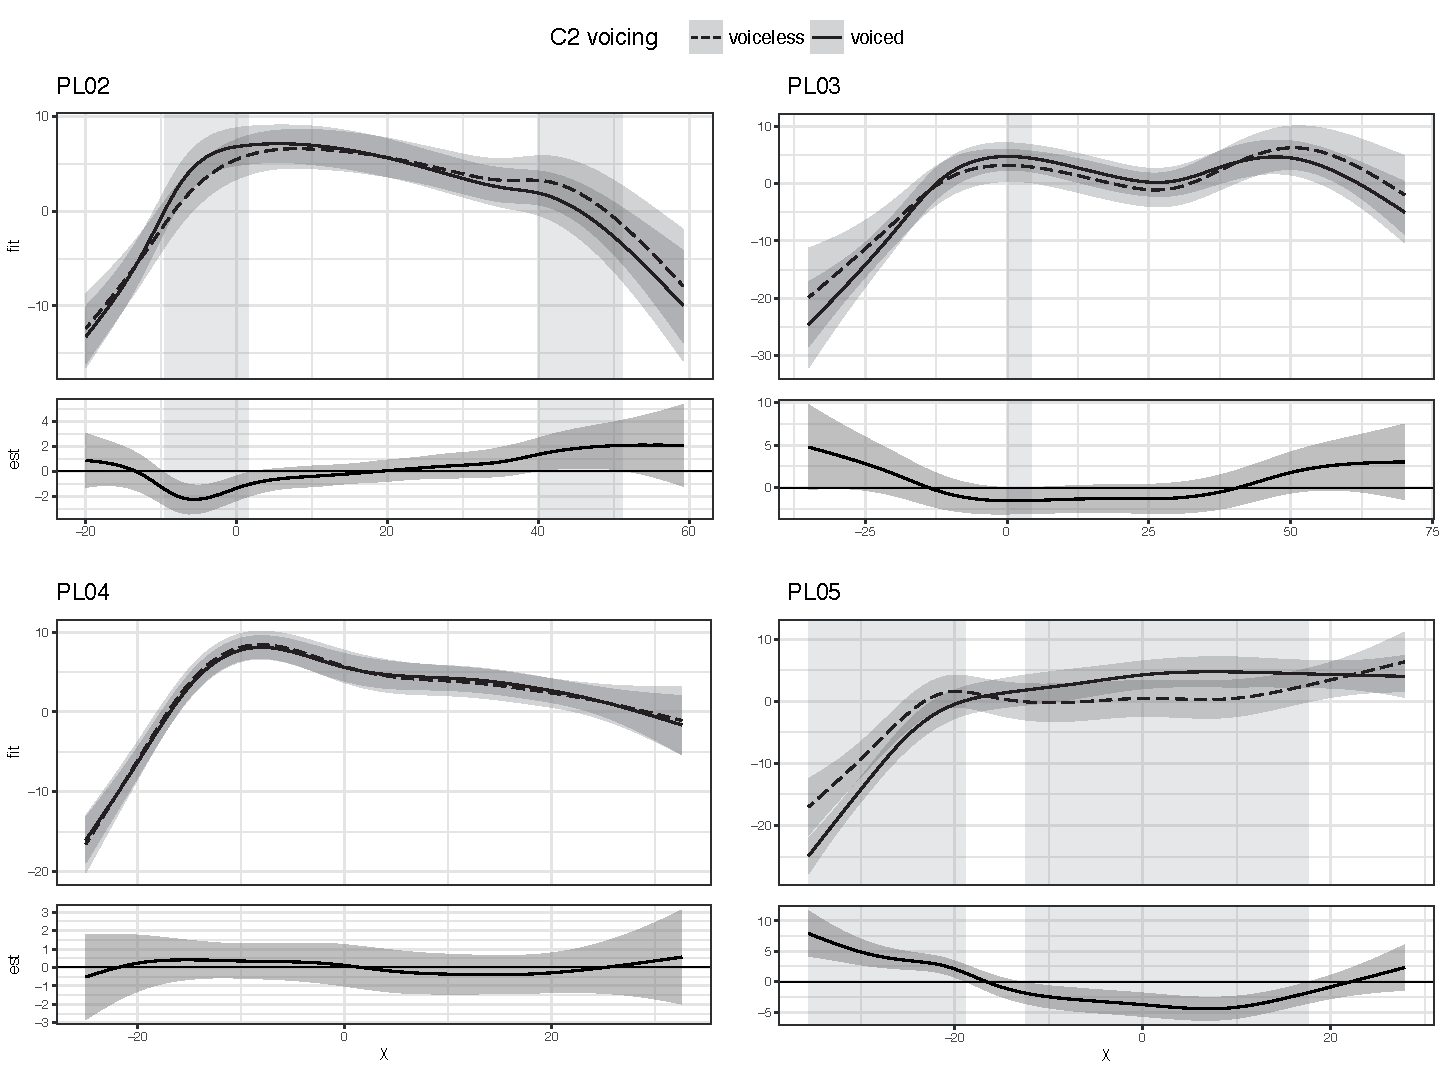
\includegraphics[width=.7\textwidth]{fig/polish-tra.pdf}
    \caption{Schematic representation of the equipment setup (\citealt{articulate2011}, see text for details).}
    \label{f:uti-setup}
\end{figure*}

Given the poor quality of the ultrasonic data for /u/, this vowel was
not included in the statistical analysis. The analysis of the Italian
ultrasonic data showed that voiced stops are produced with advancement
of the root of the tongue, as expected based on previous research on
English. Individual generalised additive mixed effect models were fitted
for each speaker: the y-coordinates of the contours were included in the
model as the outcome variable; the x-coordinates as the only parametric
term. The following smooths were specified: a reference smooth term for
the x-coordinates, three difference smooths for the x-coordinates by
\textsc{voicing}, \textsc{vowel quality}, and \textsc{place} of
articulation of the following consonant respectively, and random smooths
by word. A first-order autoregressive model was included to correct for
the high auto-correlation residuals. In two participants out of four
(IT01, IT02), the root was significantly more front in voiced stops in
both vocalic contexts (/a, o/). On the other hand, one participant
(IT03) had significant tongue root advancement only following /a/, while
the fourth participant (IT04) didn't show advancement at all. For
Polish, three out of four speakers (PL02, PL03, PL04) did not have
tongue root advancement, while the fourth speaker (PL05) had significant
advancement in voiced stops in both vocalic contexts.

Further contour analysis was carried out at C2 closure onset for Italian
and Polish speakers showing advancement. The tongue root at closure
onset was found to be already in an advanced position in voiced
consonants. Comparisons of tongue contours at C2 onset and at the time
of maximum tongue displacement in voiced consonants only further
confirmed that the degree of root advancement was larger at maximum
displacement for Italian speakers, but not for Polish.

\section{Discussion}\label{discussion}

Based on the established link between tongue root and voicing, and based
on the account by \citet{halle1967}, it was hypothesised that the
presence of the voicing effect in a language should be correlated with
the presence of tongue root advancement, if the latter plays a role in
determining the durational differences. It has been proposed that the
additional time required for the tongue to reach an advanced position in
voiced stops could be compensated for during the preceding vowel, thus
make it longer in comparison with vowels followed by voiceless stops. To
test the correlation hypothesis, ultrasonic data were collected from two
languages with and without the voicing effect, Italian and Polish
respectively.

The presence of tongue root advancement in Italian but not in Polish
provides initial support to the idea that vowels are longer if followed
by voiced stops so that enough time is allowed for the root to reach an
advanced position, prior to the consonantal closure. The reported
absence of the voicing effect in Polish could then be ascribed to the
absence of tongue root advancement in the production of voiced
consonants in this language. However, two complications derive from the
data analysed in this study. First, tongue root advancement was found in
one of the Polish speakers (PL05) on one hand and it was absent from one
of the Italian speakers (IT04) on the other. Second, vowels followed by
voiced stops in Polish were 8 milliseconds longer in Polish, contrary to
what argued in \citet{keating1984}.

However, as mentioned above, PL05 had a strikingly higher slope estimate
for the effect of voicing on vowel duration, compared to the other
speakers, meaning that the voicing effect in his data is stronger and it
is probably driving the
effect.\footnote{\label{fn:polish-small} However, note that excluding PL05 from the data yielded to an estimate of 6 milliseconds, which would still need to be explained. Given the small magnitude of the effect, it is likely that it arises from the difficulty of segmenting vowel to consonant transitions when the consonant is voiced. Such downside would not apply to the data in PL05 given the larger estimates for the effect of voicing and the random slope, as discussed above.}
Incidentally, PL05 is also the only Polish speaker who produced voiced
consonants with an advanced tongue root. Furthermore, a model comparing
tongue root at closure onset versus maximum tongue displacement in PL05
indicated that there was virtually no difference in tongue root
advancement at these two time points. Assuming the effect in the other
Polish speakers is small enough to be discarded as an artefact (see
\cref{fn:polish-small}), it follows that, independently of the language,
the presence of tongue root advancement in voiced stops correlates with
a concomitant increased duration in vowels preceding voiced consonants.

Moreover, given the smaller effect of voicing in PL05 compared to the
effect in Italian, a potential hypothesis could be that the effect of
voicing on vowel duration is gradual, rather then categorical. In this
case, even within language it should be possible to see different
magnitudes of durational differential in vowels depending on the
magnitude of advancement of the tongue root. Since the durational
difference in the polish speaker PL05 was quite small (14 milliseconds,
versus 19.5 milliseconds in Italian), one expects the magnitude of the
advancement of the root to be proportionately smaller in this speaker.
Future work will set out to investigate the hypothetic correlation
between vowel duration and amount of tongue root advancement.

Finally, the ultrasonic data showed raising of the tongue dorsum
concomitant to root advancement. The presence of such gesture, although
not expected, makes sense from an anatomical point of view. Raising of
the tongue body could be implemented as a way to counterbalance the
compression of the tongue mass caused by the advancement of the root. It
is not thus surprising to observe a raised tongue body in voiced stops
accompanying root advancement. An alternative account could ascribe
tongue body raising to aerodynamic properties of voiced stops. Since the
intra-oral pressure is higher in voiced stops due to the amount of air
needed to maintain voicing, a firmer seal at the point of oral
constriction could be used to compensate for the increased pressure.
Increasing the area of contact by raising the tongue body would provide
for a such firmer constriction.

A possible critique to the account proposed here is that, if an active
gesture for maintaining voicing is required during the closure of voiced
stops, then it is not clear how the Polish speakers without tongue root
advancement can maintain voicing. However, tongue root advancement is
not the only solution: manipulations of the larynx or of the
velopharyngeal port, rather than the tongue, can also counterbalance the
increasing intra-oral pressure {[}{]}. The gestural timing of the larynx
and the velopharyngeal port are anatomically independent (although not
completely) from the timing of tongue gestures {[}{]}, and would ideally
not require a more complex planning as with an articulatory
implementation that requires two gestures operated by the tongue.

\bibliography{linguistics.bib}

\end{document}
